\documentclass[10pt,a4paper]{article}

\usepackage[utf8]{inputenc}
\usepackage[top=0.52in,bottom=0.52in,left=0.60in,right=0.60in]{geometry}
\usepackage{amsmath,amssymb}
\usepackage{graphicx}
\usepackage{booktabs}
\usepackage{xcolor}
\usepackage{hyperref}
\usepackage{fancyhdr}
\usepackage{enumitem}
\usepackage{titlesec}

\titlespacing*{\section}{0pt}{6pt}{2pt}
\titlespacing*{\subsection}{0pt}{4pt}{1pt}

\setlength{\parskip}{0.28em}
\setlength{\parindent}{0pt}

\newenvironment{answerquote}{%
  \begin{list}{}{%
    \setlength{\leftmargin}{1.2em}%
    \setlength{\rightmargin}{1.2em}%
    \setlength{\topsep}{1.5pt}%
    \setlength{\partopsep}{0pt}%
    \setlength{\parsep}{0pt}%
    \setlength{\itemsep}{0pt}%
  }%
  \item\small\itshape
}{%
  \end{list}%
}

\definecolor{primaryblue}{RGB}{20, 45, 85}
\definecolor{accentblue}{RGB}{0, 102, 204}
\definecolor{darkgray}{RGB}{50, 50, 50}

\hypersetup{
    colorlinks=true,
    linkcolor=accentblue,
    citecolor=accentblue,
    urlcolor=accentblue
}

\pagestyle{fancy}
\fancyhf{}
\rhead{\small \textcolor{gray}{LMA Assignment 1: Baseline vs. Re-Ranking}}
\lhead{\small \textcolor{gray}{Raj K. Jain (Roll: LMA-2026)}}
\rfoot{\small Page \thepage}
\renewcommand{\headrulewidth}{0.3pt}

\begin{document}

% Title Block
\begin{center}
    {\Large \textbf{RAG Assignment 1: Dense Baseline vs. Cross-Encoder Re-Ranking}}\\[0.2ex]
    {\normalsize \textbf{Course:} Large Language Models \& AI Systems \quad$\vert$\quad \textbf{Author:} Raj K. Jain}\\[0.2ex]
    \textbf{GitHub Repository:} \url{https://github.com/Rajkjain03/lma_assignment_1}
\end{center}

\vspace{-0.9em}
\noindent\rule{\linewidth}{0.5pt}
\vspace{0.1em}

\section{Architecture Comparison: Bi-Encoder vs. Cross-Encoder}

In this assignment, I tested two retrieval pipelines for RAG: a single-stage Bi-Encoder baseline and a two-stage setup adding a Cross-Encoder re-ranker.

A \textbf{Bi-Encoder} (\texttt{all-MiniLM-L6-v2}) embeds queries and document chunks separately into 384-dimensional dense vectors, scoring relevance by cosine similarity. Because document embeddings don't depend on the query, they can be calculated once offline and indexed (e.g., using HNSW), giving fast millisecond search over large collections. But compressing an entire paragraph into a single vector inevitably loses fine details: query and passage words never interact directly during encoding, so conditions, thresholds, and negations easily get smoothed over.

A \textbf{Cross-Encoder} (\texttt{ms-marco-MiniLM-L-6-v2}) concatenates the query and passage into a single sequence and runs full transformer attention over both at once. Every query word directly attends to every word in the chunk, easily catching conditional rules (like flight duration limits) and explicit exclusions. The downside is cost: because the query and document are fused, no offline vector index can be built, requiring a full forward pass for each candidate pair at query time.

\section{Qualitative Retrieval \& Rank Shift Analysis}

\subsection{Evaluation Document \& Experimental Setup}
I built a synthetic 4-page corporate compliance manual titled \textit{``Acme Global Travel, Expense and Procurement Policy (2026)''} with 30 numbered sections. It includes realistic enterprise rules: a general coach airfare mandate with a distant exception clause, client meal guidelines placed next to distractor hotel fees, and late-submission forfeiture penalties.

To evaluate retrieval behavior, I tested six queries. Tests 1 and 2 explore distractor and context ordering effects where the target was retrieved at Rank \#3 in the baseline. Tests 3 and 4 evaluate genuine retrieval omission failures where the target clause was buried outside the Top 3 (ranks 5 and 8) in the baseline and promoted into the Top 3 by the Cross-Encoder. Tests 5 and 6 serve as controls. The generator is \texttt{Qwen/Qwen2.5-0.5B-Instruct}, a compact 0.5B parameter LLM run locally on CPU.

\begin{table}[htbp]
\centering
\small
\resizebox{\linewidth}{!}{%
\begin{tabular}{cllccc}
\toprule
\textbf{Test ID} & \textbf{Query Category} & \textbf{Target Policy Section} & \textbf{Bi-Encoder Rank} & \textbf{Cross-Encoder Rank} & \textbf{Shift} \\
\midrule
\textbf{TEST\_01} & Exceptions & Sec 2.4 (Long-Haul Flight Exception) & Rank \#3 (score: 0.4039) & \textbf{Rank \#1 (score: +0.4351)} & \textbf{+2} \\
\textbf{TEST\_02} & Distractor Chunk & Sec 5.3 (Prohibited Meal Items \& Alcohol) & Rank \#3 (score: 0.4615) & \textbf{Rank \#2 (score: +1.1171)} & \textbf{+1} \\
\textbf{TEST\_03} & Buried: Hotel Laundry & Sec 3.2 (Prohibited Hotel Incidentals) & Rank \#5 (score: 0.3667) & \textbf{Rank \#1 (score: +2.4859)} & \textbf{+4} \\
\textbf{TEST\_04} & Buried: Ancillary Fees & Sec 2.3 (Baggage \& Ancillary Airline Fees) & Rank \#8 (score: 0.3413) & \textbf{Rank \#2 (score: -1.6741)} & \textbf{+6} \\
\textbf{TEST\_05} & [CONTROL] Ground & Sec 4.4 (Luxury Chauffeured Car Ban) & Rank \#2 (score: 0.4516) & Rank \#2 (score: +1.1141) & +0 \\
\textbf{TEST\_06} & [CONTROL] Admin & Sec 8.5 (Late Submission Forfeiture) & Rank \#1 (score: 0.6565) & Rank \#1 (score: +5.2319) & +0 \\
\bottomrule
\end{tabular}%
}
\vspace{0.2em}
{\footnotesize \textit{*Note: Bi-Encoder scores are cosine similarities in $[-1, 1]$; Cross-Encoder scores are unbounded classification logits $(-\infty, +\infty)$. All values from live notebook run.}}
\caption{Retrieval rank shifts across test queries (Top 3 context cutoff).}
\label{tab:rank_shifts}
\end{table}

\begin{figure}[htbp]
\centering
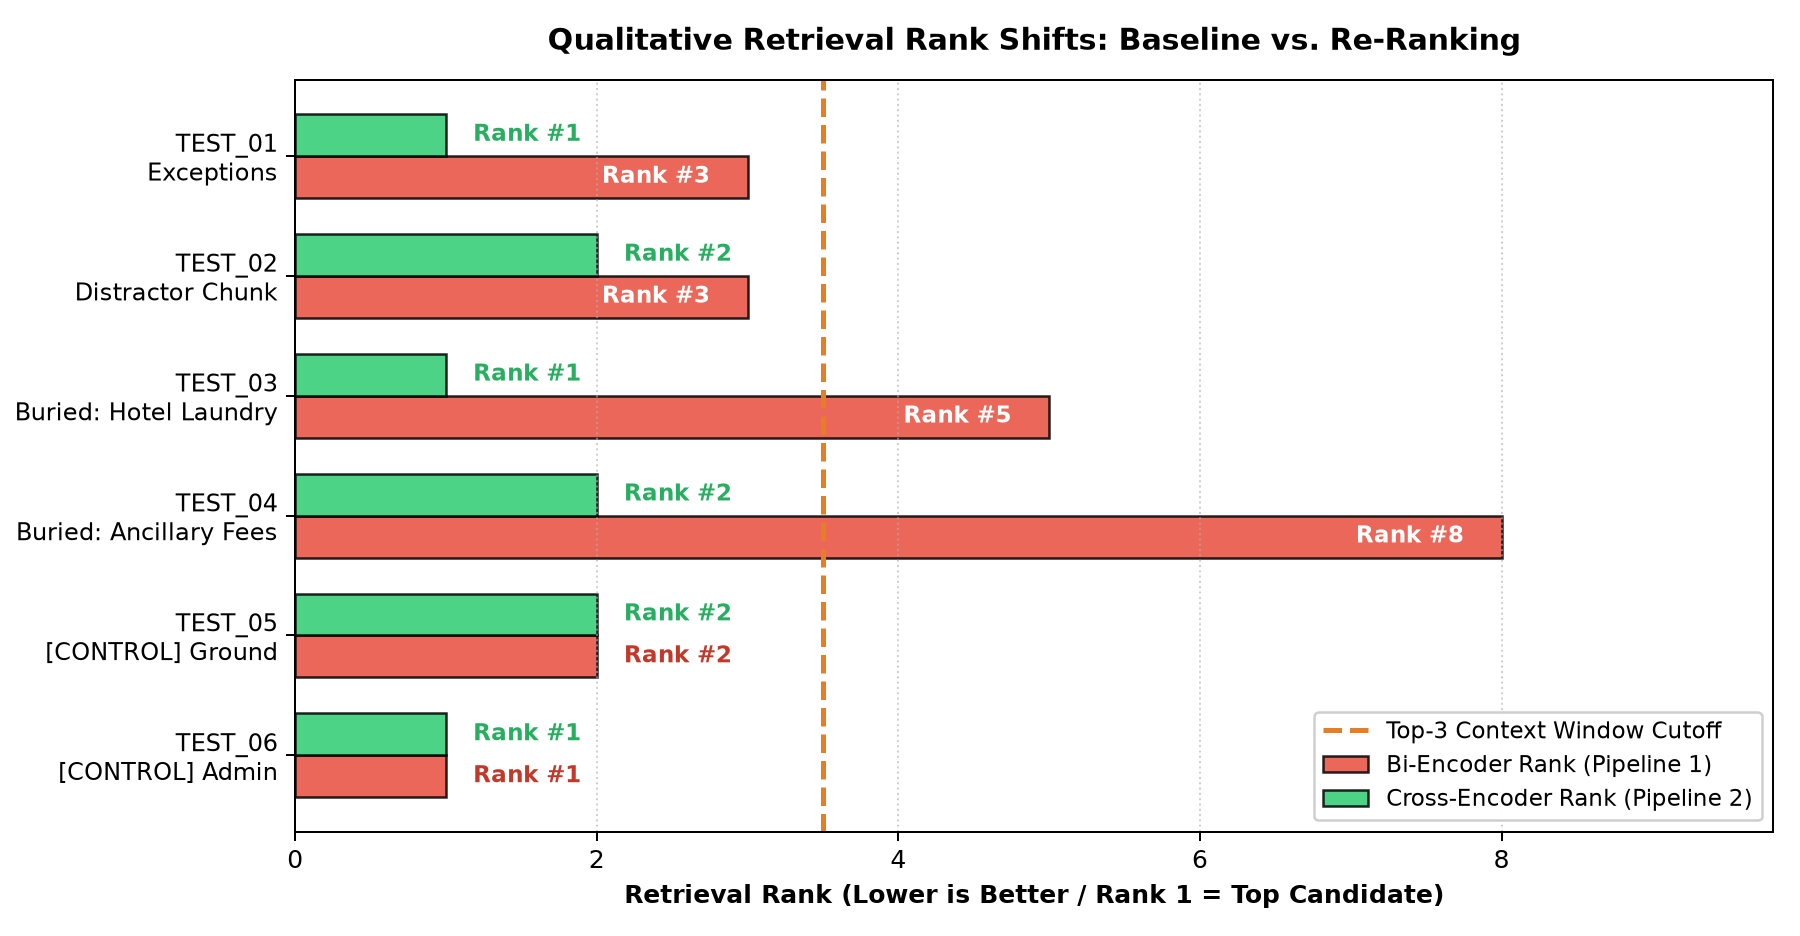
\includegraphics[width=0.73\linewidth]{rank_shifts_comparison.png}
\caption{Qualitative rank shifts: Bi-Encoder ranks (red) vs. Re-ranked Cross-Encoder ranks (green).}
\label{fig:rank_shifts}
\end{figure}

\subsection{Detailed Case Study 1: Exceptions (TEST\_01)}
\textbf{Query:} \textit{``Can staff fly in premium cabins for international client negotiations?''}\\
\textbf{Target Rule:} Section 2.4 allows Business Class on continuous non-stop international flights exceeding 8 hours (or exceeding 6 hours if presenting or negotiating within 12 hours of arrival), with written VP and CFO approval.

In baseline retrieval, Section 2.1 (\textit{Standard Cabin Class Mandate}) ranked at \#1 (cosine 0.5428), Section 1.3 was \#2 (0.4127), and Section 2.4 sat at Rank \#3 (0.4039). Because Section 2.4 was in the Top 3 context, the baseline LLM saw it. Its answer was:
\begin{answerquote}
\textbf{Answer 1 (Baseline):} \textit{``Yes, staff can fly in premium cabins for international client negotiations. However, they need to obtain prior written concurrence from both the Division Vice President and the Chief Financial Officer at least 10 business days before ticketing.''}
\end{answerquote}
Answer 1 is factually reasonable, but it missed the flight duration thresholds ($>$ 8 hours, or $>$ 6 hours for negotiations). Because our generator is a compact 0.5B model, having the coach mandate at Rank \#1 overshadowed the conditional numbers in the third chunk. A larger frontier model might have synthesized the full answer from this context, but for a 0.5B model, context ordering matters significantly. When the Cross-Encoder promoted Section 2.4 to \textbf{Rank \#1} (+0.4351), the exception sat at the front of the prompt:
\begin{answerquote}
\textbf{Answer 2 (Re-Ranked):} \textit{``Yes, staff can fly in premium cabins for international client negotiations under the long-haul international travel exception clause. The policy allows this exception when traveling on continuous non-stop international flights with flight durations exceeding 8 hours or 6 hours if the traveler is scheduled to deliver a client presentation or attend executive contract negotiations within 12 hours of flight arrival. Employees need prior written concurrence from both the Division Vice President and the Chief Financial Officer no later than 10 business days before booking their tickets.''}
\end{answerquote}

\subsection{Detailed Case Study 2: Distractor Chunk (TEST\_02)}
\textbf{Query:} \textit{``What items are not covered on expense claims for client business meals?''}\\
\textbf{Target Rule:} Section 5.3 restricts alcohol to 1 drink per diner, prohibits solo dining alcohol, and explicitly bans nightclub bottle service, adult entertainment, tobacco, and gambling losses.

In baseline retrieval, the dense retriever matched ``client business meals'' to Section 5.1 at Rank \#1 (0.5936). For the negative constraint ``not covered'', it pulled Section 3.2 (\textit{Prohibited Hotel Incidentals}) at Rank \#2 (0.5562). The actual meal prohibition clause (Section 5.3) sat at Rank \#3 (0.4615).
\begin{answerquote}
\textbf{Answer 1 (Baseline Distraction Error):} \textit{``Based on the policy context provided, the following items are not covered on expense claims for client business meals: In-room video on-demand/movie rentals, Mini-bar consumption, Laundry service for trips shorter than 5 days, Spa services, Sauna access, Dry cleaning fees, Hotel gym or fitness center pass fees...''}
\end{answerquote}
This was not an ungrounded hallucination; the 0.5B model copied items from a chunk it was given, but it was misled by a higher-ranked distractor (Section 3.2). The Cross-Encoder resolved this by recognizing that Section 5.3 directly matches meal and entertainment exclusions, promoting Section 5.3 to \textbf{Rank \#2} (+1.1171) ahead of Section 3.2:
\begin{answerquote}
\textbf{Answer 2 (Re-Ranked Corrected):} \textit{``Based on the policy context provided, the items that are not covered on expense claims for client business meals are: (a) Alcoholic beverages exceeding one (1) standard single serving of wine or beer per person during authorized client dinners. (b) Adult entertainment venues, nightclub admission or table bottle service fees, social club charges, and gentlemen's club invoices. (c) Tobacco, vape products, cannabis, and casino gambling losses. (d) Meals or travel for spouses, partners, dependents, or personal companions accompanying the traveler.''}
\end{answerquote}

\subsection{Detailed Case Studies 3 \& 4: Buried Clause Omission Failures (TEST\_03 \& TEST\_04)}
Tests 3 and 4 evaluate genuine retrieval omission failures where the target clause was buried outside the baseline Top 3 context window and rescued into the Top 3 by the Cross-Encoder.

In \textbf{TEST\_03} (\textit{``Under what trip length can travelers expense laundry and dry cleaning?''}), Section 3.2 specifies that laundry is non-reimbursable for trips shorter than 5 days. Dense search buried Section 3.2 at \textbf{Rank \#5} (0.3667), loading only filing deadlines (Section 8.1) and pre-trip authorization (Section 1.2) into the baseline prompt. Lacking the clause, the baseline LLM fabricated an answer (quoted verbatim from the notebook output):
\begin{answerquote}
\textbf{Answer 1 (Baseline Verbatim Output):} \textit{``Under the Global Travel, Expense, and Procurement Policy (2026), travelers cannot expense laundry and dry cleaning for trips longer than 30 days.''}
\end{answerquote}
Because Section 8.5 in the context mentioned 30 calendar days, the model pulled that number and invented an erroneous 30-day laundry restriction. The Cross-Encoder promoted Section 3.2 to \textbf{Rank \#1} (+2.4859), and the re-ranked model answered correctly:
\begin{answerquote}
\textbf{Answer 2 (Re-Ranked):} \textit{``For trips shorter than 5 days, travelers cannot expense laundry and dry cleaning.''}
\end{answerquote}

In \textbf{TEST\_04} (\textit{``Are flight cancellation insurance and seat selection fees reimbursable?''}), dense retrieval placed Section 2.5 (\textit{Flight Cancellations}) at \#1 and buried Section 2.3 at \textbf{Rank \#8} (0.3413) due to vocabulary mismatch. The Cross-Encoder promoted Section 2.3 to \textbf{Rank \#2} with a score of -1.6741.
\begin{answerquote}
\textbf{Answer 1 (Baseline):} \textit{``No, flight cancellation insurance and seat selection fees are not reimbursable under this policy.''}\\
\textbf{Answer 2 (Re-Ranked):} \textit{``No, flight cancellation insurance and seat selection fees are not reimbursable under this policy.''}
\end{answerquote}
Here, the Cross-Encoder score for Section 2.3 is negative (-1.6741). It reached Rank \#2 only because the other candidate chunks scored even lower (between -5 and -8). Furthermore, the query matches Section 2.3 only loosely: Section 2.3 specifies checked luggage allowances and ancillary baggage rules, but does not provide an explicit clause for flight cancellation insurance or seat selection fees. Because neither retrieval pipeline surfaced a chunk that affirmatively authorizes these fees, the generator in both pipelines produced identical negative responses. This highlights an important real-world nuance: re-ranking pushes the relatively best candidate upward, but when the underlying corpus lacks a definitive answer, the Cross-Encoder outputs negative logits and the downstream answer remains unchanged.

\subsection{Control Cases (TEST\_05 \& TEST\_06)}
In TEST\_05 (airport rideshare vs limousine ban in Section 4.4) and TEST\_06 (30-day late expense submission penalty in Section 8.5), the semantic overlap was already strong. Section 4.4 remained at Rank \#2 in both pipelines, and Section 8.5 stayed at Rank \#1 in both pipelines. These control cases verify that the Cross-Encoder does not destabilize rankings when the dense retriever already finds the correct chunk.

\section{Empirical Latency Profiling}

I benchmarked both retrieval pipelines over \textbf{10 warmed iterations} (following 5 warm-up passes to eliminate initialization noise) on my local CPU. Table~\ref{tab:latency} reports the measured runtimes.

\begin{table}[htbp]
\centering
\small
\resizebox{0.95\linewidth}{!}{%
\begin{tabular}{lcccc}
\toprule
\textbf{Test Query Category} & \textbf{P1 Baseline (Bi-Encoder)} & \textbf{Stage 2 (Cross-Encoder 10 Pairs)} & \textbf{P2 Total Latency} & \textbf{P2/P1 Overhead Ratio} \\
\midrule
\textbf{TEST\_01 (Exceptions)}      & 10.29\,ms & 129.12\,ms & 139.41\,ms & 13.55$\times$ \\
\textbf{TEST\_02 (Distractor)}      & 10.22\,ms & 143.51\,ms & 153.73\,ms & 15.04$\times$ \\
\textbf{TEST\_03 (Hotel Laundry)}   & 10.25\,ms & 126.09\,ms & 136.34\,ms & 13.30$\times$ \\
\textbf{TEST\_04 (Ancillary Fees)}  & 10.54\,ms & 154.58\,ms & 165.12\,ms & 15.67$\times$ \\
\textbf{TEST\_05 (Control: Ground)} & 10.35\,ms & 125.07\,ms & 135.42\,ms & 13.09$\times$ \\
\textbf{TEST\_06 (Control: Admin)}  & 11.26\,ms & 135.61\,ms & 146.87\,ms & 13.04$\times$ \\
\midrule
\textbf{EMPIRICAL MEAN}             & \textbf{10.48\,ms} & \textbf{135.66\,ms} & \textbf{146.15\,ms} & \textbf{13.95$\times$} \\
\bottomrule
\end{tabular}%
}
\caption{Empirical retrieval runtime profiling across 10 warmed iterations on CPU.}
\label{tab:latency}
\end{table}

\subsection{Latency Trade-Off Analysis}
The dense baseline runs in $\approx 10.5$\,ms on CPU, with roughly 9.8\,ms spent on query embedding generation and roughly 0.7\,ms on cosine dot products across the 30 chunks. Re-ranking 10 candidate pairs through the Cross-Encoder added an average of 135.7\,ms ($\approx 13.6$\,ms per candidate pair), bringing total retrieval time to $\approx 146.2$\,ms.

While a $14.0\times$ overhead sounds large, an end-to-end retrieval latency of 146\,ms remains well within the standard 200\,ms rule of thumb for interactive user search. On a dedicated GPU server, batched Cross-Encoder inference is projected to drop to an estimated 15--25\,ms total, bringing total retrieval runtime under 30\,ms.

\section{Scaling: Why Not Run Cross-Encoder Over the Whole Collection?}

If Cross-Encoders are noticeably more accurate, why not bypass the Bi-Encoder entirely and score every chunk in the collection with a Cross-Encoder?

\textbf{Compute Cost and Quadratic Complexity:} A Cross-Encoder must perform full self-attention across the concatenated sequence length $L = |q| + |c|$, which scales quadratically as $\mathcal{O}(L^2)$. Scoring a collection of $N$ passages requires running $N$ complete transformer forward passes. Based on my measured CPU runtime of 13.6\,ms per pair, evaluating a single query over a modest corporate corpus of $N = 1,000,000$ chunks would take $1,000,000 \times 13.6\,\text{ms} \approx 3.8\,\text{hours}$. Even on a modern GPU with an estimated latency of 2.0\,ms per pair, a full linear scan would take over 33 minutes per query. Under interactive user traffic, this is completely infeasible.

\textbf{Impossibility of Offline Indexing:} With a Bi-Encoder, passage embeddings are calculated once offline and indexed into sub-linear Approximate Nearest Neighbor graph structures (e.g., HNSW in FAISS), allowing millisecond search across millions of documents. In contrast, a Cross-Encoder requires both the query and passage simultaneously to compute attention. Because the query is unknown until runtime, no precomputed index can be constructed, forcing an exhaustive $\mathcal{O}(N)$ scan over every single passage.

\textbf{The Two-Stage Solution:} The two-stage funnel combines the strengths of both models: the Bi-Encoder prunes $99.999\%$ of the corpus ($1,000,000 \rightarrow 10$) in milliseconds, after which the Cross-Encoder evaluates only the top 10 candidates with joint cross-attention.

\end{document}
